% First draft. Design source of truth: docs/adr/0001-0003, issues #16-#30 on the fork.
% Quality results do not exist yet; their tables are skeletons with TBD cells.
\documentclass[10pt,twocolumn]{article}
\usepackage[letterpaper,margin=0.75in,columnsep=0.25in]{geometry}
\usepackage{times}
\renewcommand{\ttdefault}{cmtt}
\usepackage{microtype}
\usepackage{amsmath,amssymb}
\usepackage{booktabs}
\usepackage[numbers,sort&compress]{natbib}
\usepackage{xcolor}
\usepackage{tikz}
\usetikzlibrary{positioning,arrows.meta,calc,fit,patterns,decorations.pathreplacing}
\usepackage[font=small,labelfont=it,textfont=it,skip=4pt]{caption}
\usepackage{titlesec}
\usepackage{fancyhdr}
\usepackage{xspace}
\usepackage[hidelinks]{hyperref}

\setcitestyle{authoryear,round}
\titleformat{\section}{\large\bfseries\scshape}{\thesection}{0.6em}{}
\titleformat{\subsection}{\normalsize\bfseries}{\thesubsection}{0.6em}{}
\titlespacing*{\section}{0pt}{1.4ex}{0.8ex}
\titlespacing*{\subsection}{0pt}{1.1ex}{0.5ex}
\pagestyle{fancy}
\fancyhf{}
\fancyhead[C]{\small\bfseries Hierarchical Gist Trees for Long Agent Trajectories}
\fancyfoot[C]{\thepage}
\renewcommand{\headrulewidth}{0.5pt}

% placeholder name of the method; replace when the authors choose one
\newcommand{\ours}{GistTree\xspace}
\newcommand{\para}[1]{\noindent\textbf{#1}\hspace{0.5em}}
\newcommand{\tbd}{\textcolor{gray}{TBD}}
\newcommand{\sg}{\operatorname{sg}}
\newcommand{\topk}{\operatorname{TopK}_k}
\newcommand{\relmse}{\operatorname{relMSE}}

\definecolor{cpin}{RGB}{120,120,120}
\definecolor{csink}{RGB}{90,90,90}
\definecolor{craw}{RGB}{66,110,170}
\definecolor{cwin}{RGB}{110,170,110}
\definecolor{csum}{RGB}{235,190,120}
\definecolor{csel}{RGB}{40,80,150}
\definecolor{cforce}{RGB}{150,200,150}

\begin{document}

\twocolumn[
\begin{center}
{\Large\bfseries Hierarchical Gist Trees for Long Agent Trajectories:\\[2pt]
Learned Summaries, Level-wise Selective Unfolding, and On-Policy Self-Distillation\par}
\vspace{8pt}
{\normalsize Anonymous Authors\par}
\vspace{10pt}
\end{center}
]

\begin{abstract}
An agent that edits code or calls tools for hours accumulates a trajectory of 100K to 1M
tokens, appended one tool result and one response at a time. Reading the whole KV cache for
every generated token makes decoding cost grow with the trajectory. We describe \ours, which
inserts learned summary tokens (gists and meta-gists) into the sequence as it streams, so
that they form a regular 4-ary tree over the compressible history, and lets every query
unfold this tree level by level: it scores the summaries of one level, keeps a fixed number
$k$ of them, and attends to the exact tokens under the leaves it reaches. The backbone stays
frozen: only low-rank adapters on summary rows, summary embeddings and a per-summary mass
bias are trained, and raw tokens keep their original positions, so unfolding every node
reproduces the base model exactly. We train in two stages. Stage 1 distills, layer by layer,
each level of the tree into the level below it and trains selection at every position; stage
2 applies on-policy self-distillation, in which the student generates a turn through the
inference kernels and is trained by reverse KL to the full-attention base model on the same
text. The system supports appending to a live cache across turns, a two-kernel decode path
captured partly in CUDA graphs, and a training path that splits each query's keys into a
structured part computed by FlexAttention and a selected part computed by a gather kernel.
On Qwen2.5-0.5B and one H200, decoding takes 29.9\,ms per token at 128K and 30.8\,ms at 256K,
appending a 158K-token prompt takes 11\,s, and stage 1 with selection at every position
trains at 128K in 174\,s per step and 37.8\,GB. Quality results are not yet available.
\end{abstract}

% ======================================================================================
\section{Introduction}

% Spine: workload -> cost of dense decode -> selection needs good block representatives
% -> learned in-sequence summaries in a tree -> trained against the frozen base model
% -> systems work that makes append, decode and training-time selection cheap.

\para{Agent trajectories grow by appending, and most of their length is old tool output.}
A software-engineering agent starts from a fixed system prompt and tool definitions, then
alternates between a tool result (1K--50K tokens) and a response of a few hundred to a
thousand tokens. In a 200-trajectory subsample of the OpenHands trajectories we train on, the median is 50.6K tokens
\citep{badertdinov2025swerebench}, and agents that run for hours would exceed 1M. The serving
pattern is therefore not one long prefill followed by decoding, but many appends to the same
cache, each followed by a short generation.

\para{Dense attention makes every generated token read the whole trajectory.}
At 128K tokens, a dense decode step of Qwen2.5-0.5B reads about 2.1\,GB of keys and values,
and the cost grows linearly with the trajectory. Block-sparse attention reduces this by
scoring blocks of the cache and reading only the highest-scoring ones
\citep{tang2024quest,lu2025moba,yuan2025nsa}, but its quality is bounded by how well a block's
representative predicts the attention mass the block would receive. A mean-pooled key keeps
only the shared context of a block and dilutes a single salient token, which is exactly the
token a retrieval query looks for.

\para{We let the model write its own block representatives as tokens in the sequence.}
Following gist tokens \citep{mu2023gist} and Simplified Sparse Attention (SSA)
\citep{mao2026ssa}, \ours inserts a summary token after every $L=4$ raw tokens and a
higher-level summary after every $J=4$ summaries of the level below, up to $D=4$ levels.
A summary attends to the content it covers and stores the result in its own key and value;
later queries reach old content only through summaries unless they unfold them. Because
insertion depends only on position, the summaries of a prefix never change as the trajectory
grows, and the tree is a regular 4-ary tree whose layout the kernels can exploit.

\para{Selection descends the tree with a fixed beam per level.}
A query scores all top-level summaries, keeps $k$ of them, scores their children, and so on
down to the leaves, whose raw tokens it then reads exactly (Section~\ref{sec:method}). With
$k=256$, the number of keys a query reads per layer stays between 12K and 27K from 128K to
256K tokens, and the decode latency we measure is almost flat in context length
(Table~\ref{tab:decode}).

\para{The backbone is frozen, so the base model is both the teacher and the exact limit.}
Only summary rows are adapted, and raw tokens keep the RoPE positions they would have without
summaries. Unfolding every node therefore yields plain causal attention over the raw text with
the base model's weights, which we verify numerically (Section~\ref{sec:exact}). This makes
the base model a clean teacher for both training stages (Section~\ref{sec:training}).

\para{Three system components make the design trainable and servable at 128K and beyond.}
Appending to a cache uses a FlexAttention \citep{dong2024flex} mask whose keys are grouped by
summary level, which cuts a 158K-token append from 57\,s to 11\,s. Decoding uses one Triton
kernel for level-wise selection and one CUDA split-K kernel for attention over the selected
keys. Training with selection at every position splits each query's keys into a structured
part, computed by FlexAttention on full blocks, and a selected part, computed by a gather
kernel with gradients, so that time and memory grow roughly linearly up to 128K
(Section~\ref{sec:systems}).

\para{Contributions.}
We describe (i) a streaming gist tree with protected segments and a raw window suited to
appended agent trajectories, and a level-wise beam selection over it whose full expansion is
exactly the base model; (ii) a two-stage training recipe against the frozen base model,
layer-wise distillation with training-time selection followed by on-policy self-distillation
through the inference path; and (iii) the prefill, decode and training kernels that make
these practical, with their measured cost on Qwen2.5-0.5B up to 256K tokens.

% ======================================================================================
\section{Background and Related Work}
\label{sec:related}

This section fixes the facts the method relies on: how sparse methods choose what to read,
how learned compression tokens are written, how RecSA differs from our design, and why we
restrict quality targets to the base model's trained length.

\para{Block-sparse attention.}
Quest \citep{tang2024quest} scores each KV page by bounds on its keys and reads the top
pages at decode time; it needs no training but its page representative is fixed.
MoBA \citep{lu2025moba} gates blocks by the similarity between the query and the mean key
of each block; it trains the model but keeps a mean-pooled representative.
NSA \citep{yuan2025nsa} combines a compressed branch, a selected-block branch and a sliding
window, and is trained natively; its blocks form one level, so the number of scored blocks
grows linearly with context.
DSA \citep{deepseek2025dsa} scores every preceding token with a lightweight indexer and
attends to the top tokens; its indexer cost is linear in context per query.
\ours differs from all four in that the representative of a block is a token the model writes,
and blocks are organized in a tree, so the scored set per level is bounded by the beam.

\para{Learned compression tokens.}
Gist tokens \citep{mu2023gist} compress a prompt into a few tokens through an attention mask;
AutoCompressors \citep{chevalier2023autocompressors} recursively produce summary vectors for
segments; landmark attention \citep{mohtashami2023landmark} adds one token per block whose
attention score gates retrieval of the block. SSA \citep{mao2026ssa} inserts gists every $L$
tokens and meta-gists every $J$ gists, hides raw tokens behind them with a gist causal mask,
and at decode time unfolds the top-scoring chunks; it trains the full model with next-token
loss. \ours keeps SSA's insertion, mask and positions, and changes how summaries are trained
(distillation to the frozen base model instead of next-token loss), how deep the tree is, and
how selection proceeds (a fixed beam per level instead of a budget that grows with length).

\para{Recursive Sparse Attention.}
RecSA \citep{recsa2026} is the closest design. Each layer keeps a tree of keys whose node
keys are produced by a learned pooler from the keys of 16 children and whose values are the
mean of the children's values; selection descends the tree keeping $k=256$ nodes per level,
merging the heads of a GQA group by summed exponentiated scores, and the unselected candidates
stay in one softmax with the exact tokens, so summaries and tokens partition the prefix. It
places every candidate at its index in the candidate list (candidate-local RoPE), which keeps
relative distances below $Ck$ and extrapolates from 32K training to 2M, and it trains the
backbone under sparse attention at every position. Relative to RecSA, \ours computes a
summary's key and value by the backbone's own forward over the content it covers, which
makes the summary a written token rather than a pooled vector; keeps the backbone frozen and
the original positions, so full expansion is exactly the base model; uses a fanout of 4;
keeps an attention sink, protected segments and a raw window always visible; and treats
RecSA's group merge and exact partition as switches of the same selector
(Section~\ref{sec:select}). We do not adopt candidate-local positions below 256K, because they
change the relative positions of raw tokens and break exactness at full expansion.

\para{On-policy distillation.}
Distilling on sequences the student generates, with a reverse KL to the teacher, corrects the
student on the states it actually visits \citep{agarwal2024gkd,gu2024minillm}. We apply this
to a student that differs from its teacher only in what it attends to, so the teacher is the
same frozen network reading the raw text.

\para{Length extrapolation.}
RoPE \citep{su2024roformer} models degrade beyond their trained length; YaRN
\citep{peng2024yarn} rescales rotation frequencies and DCA \citep{an2024dca} remaps positions
into the trained range. Qwen2.5-7B-Instruct-1M \citep{yang2025qwen1m} is trained to 256K and
relies on DCA with YaRN beyond it. We therefore design the structure for 1M tokens but target
quality at 256K, where student and teacher both stay within trained positions.

% ======================================================================================
\section{Method: The Gist Tree and Level-wise Selective Unfolding}
\label{sec:method}

A model with $H$ query heads shares each KV head among a group $\mathcal{G}$ of $G=H/H_{kv}$
query heads \citep{ainslie2023gqa}; Qwen2.5-0.5B has $G=7$ (14 query heads, 2 KV heads) and
Qwen2.5-7B-Instruct-1M has $G=7$ (28 and 4). We describe one KV group and a query at
position $p$ of the gisted sequence, with zero-based indices.

\begin{figure*}[t]
\centering
\resizebox{\textwidth}{!}{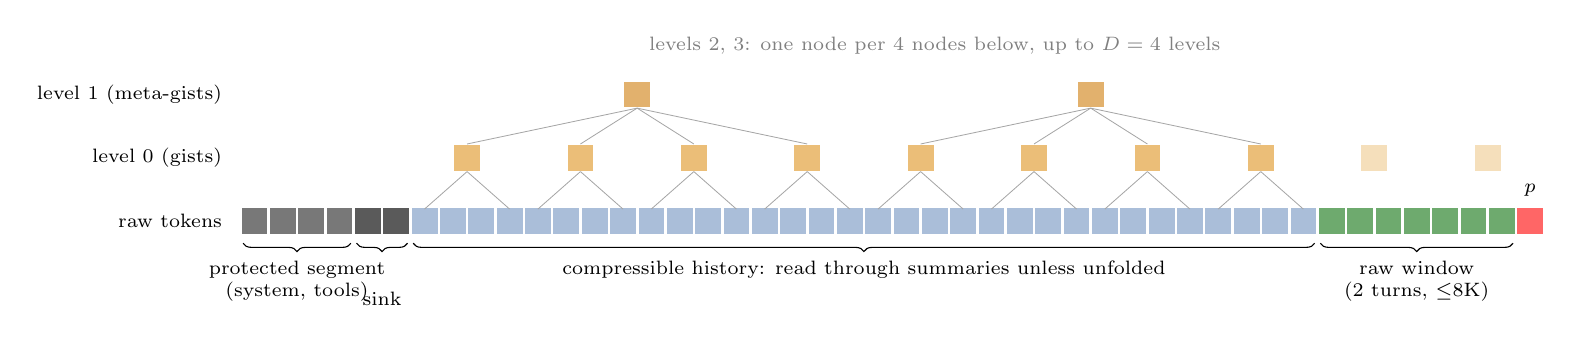
\begin{tikzpicture}[x=0.36cm,y=0.62cm,
  tok/.style={draw=white,line width=0.3pt,minimum width=0.34cm,minimum height=0.34cm,inner sep=0},
  lab/.style={font=\scriptsize,anchor=east}]
  % level 0 raw tokens: pinned 0..3, sink 4..5, compressible 6..37, window 38..45 (raw), query 46
  \foreach \i in {0,...,3} \node[tok,fill=cpin] at (\i,0) {};
  \foreach \i in {4,5} \node[tok,fill=csink] at (\i,0) {};
  \foreach \i in {6,...,37} \node[tok,fill=craw!45] at (\i,0) {};
  \foreach \i in {38,...,44} \node[tok,fill=cwin] at (\i,0) {};
  \node[tok,fill=red!60] at (45,0) {};
  \node[lab] at (-0.8,0) {raw tokens};
  % level-0 gists: one per 4 compressible tokens, 6..37 -> 8 gists (centered)
  \foreach \j in {0,...,7} {
    \pgfmathsetmacro\cx{6+4*\j+1.5}
    \node[tok,fill=csum] (g0\j) at (\cx,1.3) {};
    \draw[gray!70,line width=0.3pt] (\cx-1.5,0.25) -- (g0\j.south);
    \draw[gray!70,line width=0.3pt] (\cx+1.5,0.25) -- (g0\j.south);
  }
  % window region also has gists (inserted but invisible as unfolding is forced)
  \foreach \j in {0,1} {
    \pgfmathsetmacro\cx{38+4*\j+1.5}
    \node[tok,fill=csum!50] at (\cx,1.3) {};
  }
  \node[lab] at (-0.8,1.3) {level 0 (gists)};
  % level-1: one per 4 gists -> 2 nodes
  \foreach \j in {0,1} {
    \pgfmathsetmacro\cx{6+16*\j+7.5}
    \node[tok,fill=csum!80!brown] (g1\j) at (\cx,2.6) {};
    \foreach \c in {0,...,3} \draw[gray!70,line width=0.3pt] (g0\the\numexpr4*\j+\c\relax.north) -- (g1\j.south);
  }
  \node[lab] at (-0.8,2.6) {level 1 (meta-gists)};
  \node[font=\scriptsize,gray] at (24,3.6) {levels 2, 3: one node per 4 nodes below, up to $D=4$ levels};
  % braces
  \draw[decorate,decoration={brace,mirror,amplitude=3pt}] (-0.4,-0.45) -- (3.4,-0.45)
     node[midway,below=3pt,font=\scriptsize,align=center]{protected segment\\(system, tools)};
  \draw[decorate,decoration={brace,mirror,amplitude=3pt}] (3.6,-0.45) -- (5.4,-0.45)
     node[midway,below=14pt,font=\scriptsize]{sink};
  \draw[decorate,decoration={brace,mirror,amplitude=3pt}] (5.6,-0.45) -- (37.4,-0.45)
     node[midway,below=3pt,font=\scriptsize]{compressible history: read through summaries unless unfolded};
  \draw[decorate,decoration={brace,mirror,amplitude=3pt}] (37.6,-0.45) -- (44.4,-0.45)
     node[midway,below=3pt,font=\scriptsize,align=center]{raw window\\(2 turns, $\le$8K)};
  \node[font=\scriptsize,above=1pt] at (45,0.25) {$p$};
\end{tikzpicture}}
\caption{The gist tree of one trajectory ($L=J=4$, two of the $D=4$ levels drawn). Raw tokens
keep their order and RoPE positions. The protected segment (system prompt and tool
definitions) and the first three raw tokens after it (the attention sink) belong to no node
and are visible to every query. Every 4 compressible raw tokens are followed by a level-0
summary (gist), every 4 level-0 summaries by a level-1 summary (meta-gist), and so on; the
stream continues across segment boundaries, so a chunk may straddle a tool result and the
next response and the tree stays regular. The raw window (the last 2 turns, at most 8K
tokens) stays exact: its leaves are always unfolded, and the summaries inserted inside it
(light) only matter once it slides past them. The query $p$ (red) reads the rest of the
history through the tree (Figure~\ref{fig:select}).}
\label{fig:tree}
\end{figure*}

\subsection{Tree Construction}
\label{sec:tree}

\para{Streaming insertion.}
Summary tokens are inserted by position only. The first $s=3$ raw tokens outside protected
segments form the attention sink \citep{xiao2024sink} and are never chunked. After every
$L=4$ further raw tokens the inserter emits a level-0 summary; after every $J=4$ level-0
summaries it also emits a level-1 summary, and so on up to level $D-1=3$. Tokens of a
protected segment are passed through without counting toward a chunk. Since the rule looks
only at counts, inserting into a prefix yields a prefix of inserting into any extension, so
summaries written during one turn are never rewritten later, and the same inserter serves
training data, append prefill and decoding.

\para{Tree layout.}
The $i$-th summary of level $\ell$ is node $i$ of level $\ell$; its children are nodes
$Ji,\dots,Ji+J-1$ of level $\ell-1$, and a level-0 node covers the $L$ compressible raw tokens
before its summary. A level-$\ell$ node therefore covers $L J^{\ell}=4^{\ell+1}$ raw tokens:
4, 16, 64 and 256 for the four levels. A 128K trajectory has about 512 top-level nodes and a
1M trajectory about 4,096; the summaries add $\sum_{\ell}4^{-(\ell+1)}\approx 0.33$ tokens per
raw token. We fix $D=4$ and give each level its own embedding and bias parameters, because
the levels seen in training bound the levels usable at inference.

\para{Positions.}
Raw tokens keep the RoPE position they have without summaries, and a summary takes the
position of the raw token before it:
\begin{equation}
  \mathrm{pos}(t) \;=\; t - \sum_{t' \le t} \mathbf{1}\bigl[x_{t'}\ \text{is a summary}\bigr].
  \label{eq:pos}
\end{equation}
For $x_1\,x_2\,g_1$ this gives positions $0,1,1$. Stretching raw positions by the inserted
summaries instead would move every raw token out of its original relative distance; on
Qwen2.5-0.5B with untrained summaries fully unfolded, that alone costs 0.19 nats per token of
reverse KL to the base model, whereas Eq.~\eqref{eq:pos} gives $10^{-9}$
(Section~\ref{sec:exact}).

\para{Segments and the raw window.}
The always-visible raw tokens must have constant size, since anything visible forever is read
at every step. We keep two such parts: the protected segment of fixed length (5,707 tokens
for the system prompt and tool definitions of our data), and a raw window of the last
$N_w=2$ turns, capped at $W=8192$ tokens. Responses and tool results are compressed once they
leave the window. A segment label array, produced together with the tokens when the chat
template is rendered, marks protected tokens and turn ids; the inserter, the masks and the
kernels all read it, instead of parsing role markers in the token stream.

\subsection{Writing Summaries: the Gist Mask}
\label{sec:mask}

\para{A summary reads exactly the content it covers.}
During prefill every token attends under the gist causal mask of SSA \citep{mao2026ssa},
extended with the segments above. A level-0 summary attends to its own chunk and to the
summaries before it; a level-$\ell$ summary additionally reads its $J$ children; a summary
stays visible to later queries until a summary of the next level closes it, after which only
its parent represents it. Raw queries see their own chunk and the previous $P=1$ chunk, the
sink, the protected segment, and the raw window; summary queries are excluded from the window,
so a summary encodes only its own content. Every rule is one comparison on a few per-token
positions, so the mask is a FlexAttention \texttt{mask\_mod} with $O(T)$ features rather than
a $T\times T$ tensor.

\para{The appended part of a turn reads only summaries.}
At inference, the tokens of an appended tool result are prefilled under this mask without
unfolding; only decode rows select. Unfolding at every appended position would make prefill a
selection problem of the size of training (Section~\ref{sec:sx}). Stage 1, which selects at
every raw position, therefore differs from inference on prefill rows by design; the reasons
are given in Section~\ref{sec:stage1}.

\begin{figure}[t]
\centering
\resizebox{\columnwidth}{!}{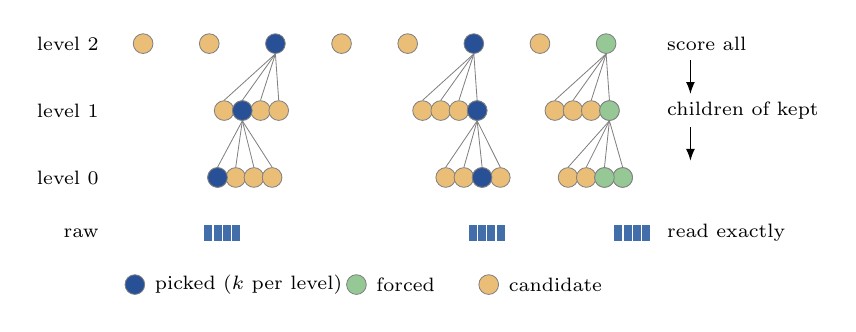
\begin{tikzpicture}[x=0.42cm,y=0.85cm,
  n/.style={circle,draw=black!50,line width=0.3pt,minimum size=0.25cm,inner sep=0},
  lab/.style={font=\scriptsize,anchor=east}]
  % top level (level 2): 8 nodes
  \foreach \i in {0,...,7} {
    \ifnum\i=2 \node[n,fill=csel] (t\i) at (\i*2+0.75,3) {};
    \else\ifnum\i=5 \node[n,fill=csel] (t\i) at (\i*2+0.75,3) {};
    \else\ifnum\i=7 \node[n,fill=cforce] (t\i) at (\i*2+0.75,3) {};
    \else \node[n,fill=csum] (t\i) at (\i*2+0.75,3) {};
    \fi\fi\fi
  }
  \node[lab] at (-0.3,3) {level 2};
  \node[font=\scriptsize,anchor=west] at (16.3,3) {score all};
  % level 1 children of 2, 5, 7
  \foreach \p/\x in {2/3.2,5/9.2,7/13.2} {
    \foreach \c in {0,...,3} {
      \node[n,fill=csum] (m\p\c) at (\x+\c*0.55,2) {};
      \draw[gray,line width=0.3pt] (t\p.south) -- (m\p\c.north);
    }
  }
  \node[n,fill=csel] at (m21) {}; \node[n,fill=csel] at (m53) {};
  \node[n,fill=cforce] at (m73) {};
  \node[lab] at (-0.3,2) {level 1};
  \node[font=\scriptsize,anchor=west] at (16.3,2) {children of kept};
  % level 0 children of m21, m53, m73
  \foreach \p/\x in {21/3.0,53/9.9,73/13.6} {
    \foreach \c in {0,...,3} {
      \node[n,fill=csum] (l\p\c) at (\x+\c*0.55,1) {};
      \draw[gray,line width=0.3pt] (m\p.south) -- (l\p\c.north);
    }
  }
  \node[n,fill=csel] at (l210) {}; \node[n,fill=csel] at (l532) {};
  \node[n,fill=cforce] at (l733) {}; \node[n,fill=cforce] at (l732) {};
  \node[lab] at (-0.3,1) {level 0};
  % raw tokens under selected leaves
  \foreach \p/\x in {210/2.6,532/10.6,733/15.0} {
    \foreach \c in {0,...,3} \fill[craw] (\x+\c*0.28,0.05) rectangle ++(0.24,0.24);
  }
  \node[lab] at (-0.3,0.17) {raw};
  \node[font=\scriptsize,anchor=west] at (16.3,0.17) {read exactly};
  \draw[-{Latex[length=1.5mm]},line width=0.4pt] (17.3,2.75) -- (17.3,2.25);
  \draw[-{Latex[length=1.5mm]},line width=0.4pt] (17.3,1.75) -- (17.3,1.25);
  % legend
  \node[n,fill=csel,label={[font=\scriptsize]right:picked ($k$ per level)}] at (0.5,-0.6) {};
  \node[n,fill=cforce,label={[font=\scriptsize]right:forced}] at (7.2,-0.6) {};
  \node[n,fill=csum,label={[font=\scriptsize]right:candidate}] at (11.2,-0.6) {};
\end{tikzpicture}}
\caption{Level-wise selection for one query and one KV group ($k=2$ drawn; $k=256$ by
default). The query scores every closed top-level node (Eq.~\eqref{eq:score}) and keeps $k$
free nodes (dark) plus the forced nodes (green), the ancestors of the leaves the query
already sees exactly (its previous chunk and the raw window). The closed children of the kept
nodes form the candidates of the next level, which are scored and cut to $k$ again. At level
0 the kept leaves are unfolded: the query reads their raw tokens. Without coarse terms the
summaries of the kept nodes stay visible as well (SG+SR); with coarse terms the unkept
candidates (orange) enter the softmax instead and the kept nodes are replaced by their
children (Eq.~\eqref{eq:visible}).}
\label{fig:select}
\end{figure}

\subsection{Level-wise Beam Selection}
\label{sec:select}

\para{Scores.}
Query head $h\in\mathcal{G}$ scores the summary token $g^{(\ell)}_i$ of node $i$ at level
$\ell$ by its attention logit plus a learned per-summary mass bias $\beta$
(Section~\ref{sec:params}):
\begin{equation}
  s^{(\ell)}_{h,i}(p) \;=\; \frac{\mathbf{q}_{p,h}^{\top}\mathbf{k}_{g^{(\ell)}_i}}{\sqrt{d}}
  \;+\; \beta_{g^{(\ell)}_i},
  \label{eq:score}
\end{equation}
where $\mathbf{q}_{p,h}$ and $\mathbf{k}$ are rotated by RoPE at their positions from
Eq.~\eqref{eq:pos} and $d$ is the head dimension. The same bias enters the attention logit
of the summary, so the score that selects a node and the logit that weighs it agree.

\para{Candidates.}
Let $\mathcal{N}^{(\ell)}(p)$ be the level-$\ell$ nodes closed before $p$ (their summary
precedes $p$), and $n_\ell=|\mathcal{N}^{(\ell)}(p)|$. The top level offers all its closed
nodes; below it, a closed node is a candidate if its parent was kept, or if its parent is not
yet closed (it lies on the query's own open path, so the region after the last top-level
summary remains reachable):
\begin{equation}
\begin{aligned}
  \mathcal{A}^{(D-1)} &= \mathcal{N}^{(D-1)},\\
  \mathcal{A}^{(\ell)} &= \bigl\{\, i\in\mathcal{N}^{(\ell)} :
     \lfloor i/J \rfloor \in \mathcal{S}^{(\ell+1)} \ \text{or}\
     \lfloor i/J \rfloor \ge n_{\ell+1} \bigr\}.
\end{aligned}
\label{eq:cand}
\end{equation}

\para{Forced nodes.}
The gist mask already shows the query some raw tokens exactly: its previous chunk and the
raw window. Let $\lambda(p)$ be the lowest leaf containing such a token. Those leaves and
their ancestors are kept without counting against $k$,
$\mathcal{F}^{(\ell)}=\{i\in\mathcal{N}^{(\ell)}: i\ge\lfloor\lambda(p)/J^{\ell}\rfloor\}$,
which keeps the visible set below a partition of the history when coarse terms are on.

\para{Selection.}
Each level keeps the forced nodes and $k$ free candidates:
\begin{equation}
  \mathcal{S}^{(\ell)} \;=\; \mathcal{F}^{(\ell)} \,\cup\,
  \operatorname{Pick}_k\!\bigl(\mathcal{A}^{(\ell)}\setminus\mathcal{F}^{(\ell)}\bigr),
  \label{eq:sel}
\end{equation}
for $\ell=D-1,\dots,0$, with ties broken toward the lower node id. The group merge is a
switch. \emph{Union} keeps a node if any head ranks it in its own top $k$,
$\operatorname{Pick}_k=\bigcup_{h\in\mathcal{G}}\topk(\{s^{(\ell)}_{h,i}\}_i)$, as in SSA's
grouped unfolding; \emph{sumexp} ranks the group's importance
$I_i=\sum_{h\in\mathcal{G}}\exp(s^{(\ell)}_{h,i})$ once, as in RecSA. Union keeps between $k$
and $Gk$ nodes; on Qwen2.5-0.5B with $G=7$ and $k=256$ it keeps 400--1,100 nodes per level,
while sumexp keeps exactly 256. Union is the current default; the choice is part of the
quality study.

\subsection{One Softmax over Exact Tokens and Summaries}
\label{sec:softmax}

\para{Visible set.}
The query attends to the always-visible tokens $\mathcal{R}(p)$ (protected segment and sink),
the raw tokens of kept and open leaves, and a set of summaries $\Sigma(p)$:
\begin{equation}
\begin{aligned}
  \mathcal{V}(p) &= \mathcal{R}(p) \cup \mathcal{U}(p) \cup \Sigma(p),\\
  \mathcal{U}(p) &= \bigl\{ j : \mathrm{leaf}(j)\in\mathcal{S}^{(0)}\ \text{or}\
     \mathrm{leaf}(j)\ge n_0 \bigr\},\\
  \Sigma(p) &= \textstyle\bigcup_{\ell}
     \begin{cases}
       g\bigl(\mathcal{S}^{(\ell)}\bigr) & \text{(SG+SR)},\\
       g\bigl(\mathcal{A}^{(\ell)}\setminus\mathcal{S}^{(\ell)}\bigr) & \text{(coarse terms)},
     \end{cases}
\end{aligned}
\label{eq:visible}
\end{equation}
where $j$ ranges over compressible raw tokens before $p$, $g(\cdot)$ maps nodes to their
summary tokens, and the first case of $\Sigma$ holds without coarse terms, the second with
them. Head $h$ then computes
\begin{equation}
  \mathbf{o}_{p,h} \;=\; \sum_{j\in\mathcal{V}(p)}
   \frac{\exp(s_{h,j})}{\sum_{j'\in\mathcal{V}(p)}\exp(s_{h,j'})}\,\mathbf{v}_j,
  \label{eq:attn}
\end{equation}
with $s_{h,j}$ the logit of Eq.~\eqref{eq:score} and $\beta_j=0$ for raw tokens.

\para{Coarse terms make the summaries and tokens an exact partition.}
With coarse terms, a kept node contributes only its children and an unkept candidate only its
own summary, so every compressible raw token is represented exactly once, as in RecSA. Without
them, a kept node's summary is visible next to its unfolded content, which is SSA's SG+SR rule
and counts that content's mass twice; it is the default only because it keeps the existing
SSA path unchanged. Unkept candidates receive gradient from the task loss only when coarse
terms are on.

\para{Full expansion is the base model.}
If every candidate is kept, Eq.~\eqref{eq:visible} with coarse terms contains no summaries and
all raw tokens before $p$, so Eq.~\eqref{eq:attn} is causal attention over the raw text. Since
raw rows use the base weights (Section~\ref{sec:params}) and the original positions
(Eq.~\eqref{eq:pos}), the student then equals the base model, and any measured deviation is a
bug rather than a modeling error.

\para{Cost.}
At each level a query scores at most $J|\mathcal{S}^{(\ell+1)}|$ candidates below the top and
$n_{D-1}$ at the top, so selection cost depends on the beam, not on the context below the top
level. The keys read per layer are the protected segment, the sink, the window, $L$ raw tokens
per kept leaf, and the visible summaries; on Qwen2.5-0.5B at 128K this is 12K--15K keys per
layer and KV group, against about 175K for dense attention over the gisted sequence.

% ======================================================================================
\section{Training}
\label{sec:training}

\subsection{What Is Trained}
\label{sec:params}

\para{Only summary rows are adapted.}
Each attention projection $W\in\{W_Q,W_K,W_V,W_O\}$ becomes $W+BA$ on summary rows only, with
rank $r=32$ LoRA \citep{hu2022lora} factors ($B$ initialized to zero) shared across levels,
and raw rows use $W$ unchanged; the MLP is shared. In the last layer only $W_K$ and $W_V$ are
adapted, since its summary queries and outputs feed no loss. The trainable parameters are
these adapters, one embedding per summary level, and the mass bias. Three properties follow.
Raw tokens compute exactly what the base model computes, which gives exactness at full
expansion. Switching the adapters off recovers the teacher without a second copy of the
weights. And the student cannot lower a distillation loss by changing raw queries so that they
stop looking far away, a degenerate solution available to any method that adapts raw rows.

\para{Each summary carries its own mass bias.}
A single key cannot express how much attention mass a node's subtree would receive: the mass
is a log-sum-exp over its raw keys and depends on how spread they are. For a level-$\ell$
summary at position $t$, each KV head has
\begin{equation}
  \beta_t \;=\; b_\ell + \mathbf{u}_\ell^{\top}\,\mathrm{RMSNorm}(\mathbf{h}_t),
  \label{eq:beta}
\end{equation}
where $\mathbf{h}_t$ is the attention input of the summary row, $b_\ell$ starts at
$\log(LJ^{\ell})$, the number of raw tokens the level covers, and $\mathbf{u}_\ell$ at zero.
The initial value follows from
$\log\sum_{j}\exp(\mathbf{q}^\top\mathbf{k}_j)\ge\log n+\mathbf{q}^\top\bar{\mathbf{k}}$ for
$n$ keys with mean $\bar{\mathbf{k}}$. A per-level scalar would be constant within a level's
softmax and receive no gradient from a routing loss over that level. Layer 0 has no bias and
uses plain gist-mask attention at inference; it takes no part in selection.

\begin{figure*}[t]
\centering
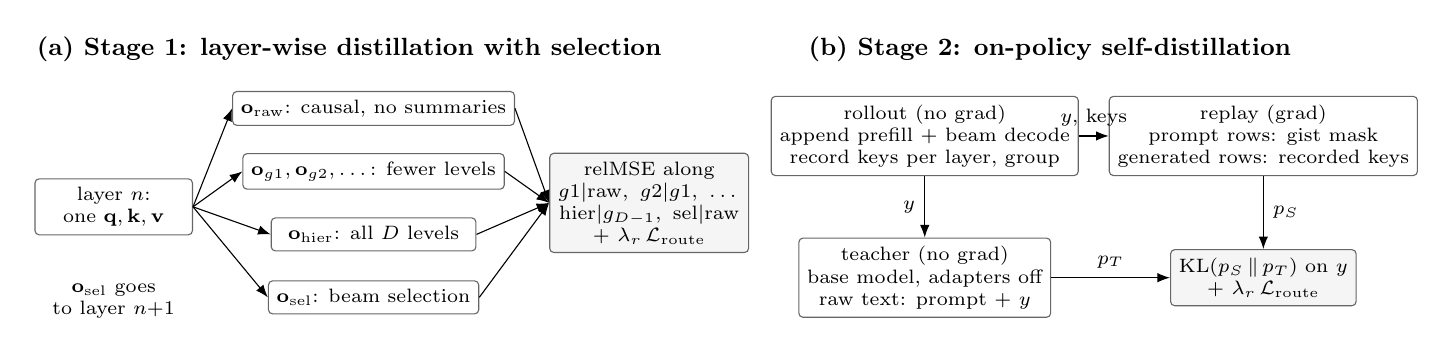
\begin{tikzpicture}[font=\scriptsize,
  box/.style={draw=black!60,line width=0.4pt,rounded corners=1.5pt,align=center,inner sep=3pt},
  arr/.style={-{Latex[length=1.6mm]},line width=0.4pt}]
  % Stage 1
  \node[font=\small\bfseries,anchor=west] at (0,3.0) {(a) Stage 1: layer-wise distillation with selection};
  \node[box,minimum width=2.0cm] (qkv) at (1.1,1.0) {layer $n$:\\one $\mathbf{q},\mathbf{k},\mathbf{v}$};
  \node[box,minimum width=2.6cm] (raw) at (4.4,2.25) {$\mathbf{o}_{\text{raw}}$: causal, no summaries};
  \node[box,minimum width=2.6cm] (g1)  at (4.4,1.45) {$\mathbf{o}_{g1},\mathbf{o}_{g2},\dots$: fewer levels};
  \node[box,minimum width=2.6cm] (hier) at (4.4,0.65) {$\mathbf{o}_{\text{hier}}$: all $D$ levels};
  \node[box,minimum width=2.6cm] (sel) at (4.4,-0.15) {$\mathbf{o}_{\text{sel}}$: beam selection};
  \foreach \t in {raw,g1,hier,sel} \draw[arr] (qkv.east) -- (\t.west);
  \node[box,fill=gray!8] (loss1) at (7.9,1.05) {$\relmse$ along\\$g1|\text{raw},\ g2|g1,\ \dots$\\$\text{hier}|g_{D-1},\ \text{sel}|\text{raw}$\\$+\ \lambda_r\,\mathcal{L}_{\text{route}}$};
  \foreach \t in {raw,g1,hier,sel} \draw[arr] (\t.east) -- (loss1.west);
  \node[font=\scriptsize,align=center] at (1.1,-0.2) {$\mathbf{o}_{\text{sel}}$ goes\\to layer $n{+}1$};
  % Stage 2
  \node[font=\small\bfseries,anchor=west] at (9.8,3.0) {(b) Stage 2: on-policy self-distillation};
  \node[box] (roll) at (11.4,1.9) {rollout (no grad)\\append prefill + beam decode\\record keys per layer, group};
  \node[box] (teach) at (11.4,0.1) {teacher (no grad)\\base model, adapters off\\raw text: prompt + $y$};
  \node[box] (rep) at (15.7,1.9) {replay (grad)\\prompt rows: gist mask\\generated rows: recorded keys};
  \node[box,fill=gray!8] (loss2) at (15.7,0.1) {$\mathrm{KL}(p_S\,\|\,p_T)$ on $y$\\$+\ \lambda_r\,\mathcal{L}_{\text{route}}$};
  \draw[arr] (roll) -- node[above]{$y$, keys} (rep);
  \draw[arr] (roll) -- node[left]{$y$} (teach);
  \draw[arr] (rep) -- node[right]{$p_S$} (loss2);
  \draw[arr] (teach) -- node[above]{$p_T$} (loss2);
\end{tikzpicture}
\caption{The two training stages. (a) Stage 1 runs one forward pass; at every layer the same
queries, keys and values are attended under several masks: plain causal attention over the
raw tokens, the tree truncated to fewer levels, the full tree, and the full tree with
level-wise selection at every raw position. Each student output is matched to the output one
compression step less lossy (relative MSE after $W_O$, teacher detached), and $\mathbf{o}_{\text{sel}}$
is passed to the next layer; $\mathbf{o}_{\text{hier}}$ appears only inside the teacher-chain losses. A routing KL fits the summary scores
to the true attention mass of their subtrees. (b) Stage 2 samples a response $y$ from the
student through the inference path, recording the keys each layer and KV group attended to;
the frozen base model scores $y$ on the raw text; the replay recomputes the student's
distribution on $y$ with gradient, attending to exactly the recorded keys, and is trained by
reverse KL to the teacher plus the routing KL.}
\label{fig:training}
\end{figure*}

\subsection{Stage 1: Layer-wise Distillation along a Teacher Chain}
\label{sec:stage1}

\para{Each level learns to compress the level below it.}
In one forward pass, layer $n$ computes its queries, keys and values once and attends under a
set of masks $m$: \textit{raw} (causal attention over raw tokens, no summaries), $g_m$ (the
tree truncated to $m$ levels, so distant content is read through level-$(m-1)$ summaries),
\textit{hier} (all $D$ levels), and \textit{sel} (the full tree with the selection of
Section~\ref{sec:select} at every raw position). The loss matches each student output to a
detached teacher output one compression step less lossy:
\begin{equation}
\begin{aligned}
  \mathcal{L}_1 = {}&\sum_{n}\sum_{(a,b)\in\Pi}
     \relmse\bigl(W_O\mathbf{o}^{[n]}_a,\ \sg(W_O\mathbf{o}^{[n]}_b)\bigr)\\
     &+ \lambda_r\,\mathcal{L}_{\text{route}},
\end{aligned}
  \label{eq:stage1}
\end{equation}
with $\Pi$ the pairs $(g_1,\text{raw})$, $(g_2,g_1)$, \dots, $(\text{hier},g_{D-1})$ and
$(\text{sel},\text{raw})$, and $\relmse(\mathbf{a},\mathbf{b})$ the mean over loss rows of
$\|\mathbf{a}_t-\mathbf{b}_t\|^2/\|\mathbf{b}_t\|^2$. Loss rows are raw, unpadded, unprotected
tokens past the sink. With selection on (the adopted configuration), the output passed to the
next layer is $\mathbf{o}_{\text{sel}}$, so later layers see the inputs that decode-time selection
produces, and $\mathbf{o}_{\text{hier}}$ appears only inside the teacher-chain losses; without
selection, $\mathbf{o}_{\text{hier}}$ is passed down. Teachers are local to the layer and inherit
upstream compression error; gradients flow
across layers, because the write side of a summary ($W_Q$, $W_O$ on summary rows) receives
gradient only from the losses of later layers.

\para{Training-time selection was adopted after a pre-registered gate.}
The \textit{sel} pair trains the summaries under the same selection the model uses at decode
time; the selected indices carry no gradient. We added it after a controlled comparison on
Qwen2.5-0.5B at 8K, with thresholds fixed in advance (a 20\% lower suffix KL, or 10 points
more passkey accuracy for keys in the first half of the context). The outcome is reported
with the quality results (Table~\ref{tab:gate}); a repeat at 32K on agent trajectories is in
progress.

% Pending the 32K repeat of the gate (#29), which is under investigation for a training bug.
% Preliminary 8K values (#28, ADR 0003): A->B in training lowers suffix KL by 47%; selecting at
% prefill as well changes it by 5-7%.
\para{Selection is trained at every position but used at decode only.}
At inference, prefill rows keep the gist mask (summaries plus forced raw tokens) and only
decode rows select, so stage 1 deliberately differs from inference on prefill rows. In the 8K
gate the gain came from training: switching training from no selection to selection at every
position lowered the suffix KL by \tbd\%, whereas also selecting at prefill rows at inference
changed it by only \tbd\%, too little to justify a selection kernel for prefill.

\para{The beam scales with context so that the selected fraction stays comparable.}
Training uses $k=16$ and inference $k=256$. At 32K with $D=4$ the top level has
$32768/4^4=128$ nodes, so $k=256$ would keep all of them and there would be no selection at
training time; $k=16$ keeps 1/8. At 1M the top level has 4,096 nodes and $k=256$ keeps 1/16.

\para{Routing KL supervises every summary, selected or not.}
For a sampled query row and level $\ell$, the label is the softmax, over the candidate units,
of the log-sum-exp of the query's logits on each unit's raw keys; the prediction is the
softmax of the scores of Eq.~\eqref{eq:score} over the same units:
\begin{equation}
\begin{aligned}
  y^{(\ell)}_{h,i} &= \operatorname{softmax}_i\Bigl(\log\textstyle\sum_{j\in i}e^{s_{h,j}}\Bigr),\\
  \pi^{(\ell)}_{h,i} &= \operatorname{softmax}_i\bigl(s^{(\ell)}_{h,i}\bigr),\\
  \mathcal{L}_{\text{route}} &= \frac{1}{|\mathcal{H}|}\sum_{(p,h,\ell)\in\mathcal{H}}
   \mathrm{KL}\bigl(\mathbf{y}^{(\ell)}_{h}\,\big\|\,\boldsymbol{\pi}^{(\ell)}_{h}\bigr),
\end{aligned}
  \label{eq:route}
\end{equation}
where $\mathcal{H}$ ranges over 32 sampled rows per sequence, all heads and levels; the protected segment and the sink
belong to no unit, since the sink alone holds 25--45\% of the mass in middle and late layers.
A variant restricts the units below the top to the children of the highest-mass parents,
matching the comparison selection actually makes.

\subsection{Stage 2: On-Policy Self-Distillation}
\label{sec:opsd}

\para{The student is trained on the states it visits at inference.}
A training step cuts a trajectory where an assistant turn begins, and the student appends the
prompt and samples the turn through the inference path of Section~\ref{sec:systems}. At every
fed token, each layer records the key positions it attended to for each KV group. The teacher
is the same network with adapters off, reading the raw prompt and response without summaries;
raw tokens share positions on both sides, so the two align token by token. The replay
recomputes the response with gradient in one parallel forward pass in which response rows
attend to exactly the recorded keys:
\begin{equation}
\begin{aligned}
  \mathcal{L}_2 = {}&\frac{1}{|Y|}\sum_{t\in Y}
   \mathrm{KL}\bigl(p_S(\cdot\mid y_{<t})\,\big\|\,p_T(\cdot\mid y_{<t})\bigr)\\
   &+ \lambda_r\,\mathcal{L}_{\text{route}},
\end{aligned}
  \label{eq:opsd}
\end{equation}
with $Y$ the generated raw tokens, the reverse KL over the full vocabulary, and $\lambda_r=0.1$.

\para{Recording keys, not re-selecting, keeps replay faithful.}
Incremental decoding and a parallel forward pass agree only to floating-point tolerance, so
re-running selection in the replay would flip near-tied nodes; replaying the recorded key sets
removes that source of mismatch. In fp32 the replayed and sampled log-probabilities differ by
at most $10^{-4}$; in bf16 at 128K they differ by about 0.04 on average, with identical key
sets. Reverse KL reaches only the summaries the student attended to (and, with coarse terms,
the unkept siblings); the routing KL reaches all of them. We distill on single turns without
executing tools; multi-turn rollouts with a sandbox are left for later.

% ======================================================================================
\section{Efficient Prefill, Decoding and Training}
\label{sec:systems}

\subsection{Append Prefill}
\label{sec:prefill}

\para{A session appends to one cache across turns.}
A session holds the KV cache, the inserter state and the segment labels. Appending a tool
result inserts summaries by the streaming rule, continuing from the previous append, and
prefills the new rows against the whole cache with FlexAttention, using a block mask with a
query offset and the $O(T)$ mask features of Section~\ref{sec:mask}. Appending in pieces is
allclose to prefilling everything at once. A 128K-token trajectory (175K with summaries)
appended in four pieces peaks at 4.46\,GB on Qwen2.5-0.5B, below the 7.6\,GB a single dense
mask of that size would take.

\para{Grouping summary keys by level makes almost every block full or empty.}
In sequence order, summaries of all levels interleave, so every key block over old content
holds a few visible top-level summaries among many invisible lower-level ones, and FlexAttention
must evaluate the mask on every element of such partial blocks. We permute keys as
$[\,\text{raw}\mid\text{level }0\mid\text{level }1\mid\cdots\,]$, each in position order; within a
level, the summaries a query sees are then one contiguous run. On a 158K-token agent prompt,
partial blocks fall from 27.6\% to 5.2\% of the causal grid and the append from 57.1\,s to
11.1\,s (Table~\ref{tab:prefill}). The output is unchanged up to summation order (fp32 relative
error at most $8.4\times10^{-6}$).

\begin{figure*}[t]
\centering
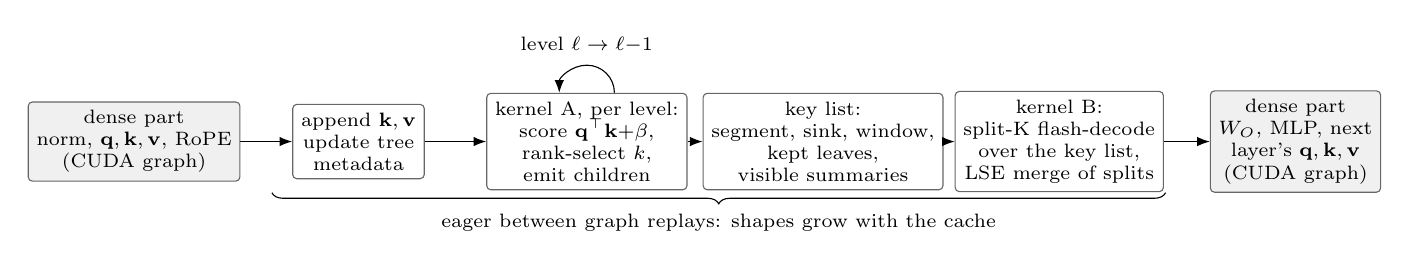
\begin{tikzpicture}[font=\scriptsize,
  box/.style={draw=black!60,line width=0.4pt,rounded corners=1.5pt,align=center,inner sep=3pt,minimum height=0.9cm},
  gbox/.style={box,fill=gray!12},
  arr/.style={-{Latex[length=1.6mm]},line width=0.4pt}]
  \node[gbox] (d0) at (0,0) {dense part\\norm, $\mathbf{q},\mathbf{k},\mathbf{v}$, RoPE\\(CUDA graph)};
  \node[box] (kv) at (2.85,0) {append $\mathbf{k},\mathbf{v}$\\update tree\\metadata};
  \node[box] (A) at (5.75,0) {kernel A, per level:\\score $\mathbf{q}^\top\mathbf{k}{+}\beta$,\\rank-select $k$,\\emit children};
  \node[box] (list) at (8.75,0) {key list:\\segment, sink, window,\\kept leaves,\\visible summaries};
  \node[box] (B) at (11.75,0) {kernel B:\\split-K flash-decode\\over the key list,\\LSE merge of splits};
  \node[gbox] (d1) at (14.75,0) {dense part\\$W_O$, MLP, next\\layer's $\mathbf{q},\mathbf{k},\mathbf{v}$\\(CUDA graph)};
  \draw[arr] (d0) -- (kv); \draw[arr] (kv) -- (A); \draw[arr] (A) -- (list);
  \draw[arr] (list) -- (B); \draw[arr] (B) -- (d1);
  \draw[arr] (A.north) ++(0.35,0) arc[start angle=0,end angle=180,radius=0.35] node[above=1pt,pos=0.5]{level $\ell\to\ell{-}1$};
  \draw[decorate,decoration={brace,mirror,amplitude=4pt}] (1.75,-0.65) -- (13.1,-0.65)
     node[midway,below=4pt]{eager between graph replays: shapes grow with the cache};
\end{tikzpicture}
\caption{One layer of a decode step for a raw token. The dense parts of consecutive layers
(output projection, MLP, normalization, query/key/value projections and RoPE) have static
shapes and are replayed as CUDA graphs. Between them run the cache update and incremental
tree metadata, kernel A (Triton), which scores each level's candidates for every head of every
KV group, keeps $k$ by rank selection and emits the next level's candidates, a kernel that
assembles each group's key list, and kernel B (CUDA), a split-K flash-decode over that list
with a per-key bias ($\beta$ on summaries). The kept node ids are recorded when the step is part
of an OPSD rollout. Summary rows emitted after a raw token are fed through the same kernel B
with their gist-mask key list, outside the graphs.}
\label{fig:decode}
\end{figure*}

\subsection{Decoding}
\label{sec:decode}

\para{Kernel A selects without sorting.}
For each level, one Triton \citep{tillet2019triton} program per query head computes the scores
of Eq.~\eqref{eq:score} for its candidates into a small scratch buffer, finds the $k$-th largest
score by a 32-pass bitwise count, and resolves ties at the threshold toward lower node ids by
a prefix sum; union ORs the heads' picks with atomics, so the result does not depend on
program order, and sumexp ranks the summed exponentiated scores. A second Triton kernel turns
the kept nodes into the next level's candidates with a prefix sum instead of sorting. Moving
from one program per KV group to one per head cut the pick from 0.24\,ms to 0.025\,ms per level
and the GPU time of a 158K decode step from 41\,ms to 22\,ms.

\para{Kernel B reads only the listed keys.}
A Triton kernel writes, for each KV group, one list of key positions: the protected segment,
the sink, the window, the raw tokens of kept and open leaves, and the visible summaries.
Kernel B, in CUDA, runs split-K flash-decoding \citep{dao2023flashdecoding} over the list with
about 128 keys per split, adds the per-key bias, and merges splits by log-sum-exp; the head
dimension and heads per group are template parameters (64 and 128; up to 8). Layer 0 and
summary rows use the same kernel with their gist-mask key lists.

\para{Tree metadata is maintained incrementally.}
An incremental structure keeps, token by token, the summary positions and closed counts per
level, the four raw positions of each leaf, the always-visible positions and the lowest forced
leaf, in amortized $O(1)$ per token. Rebuilding the tree each step had cost $O(T)$ and
dominated the step at 128K (0.32\,s to 0.08\,s per step).

\para{CUDA graphs cover the static part of each layer.}
The attention part changes shape every step (cache length, candidate counts, key list
length), so we capture only the dense parts between attentions, one graph per layer boundary,
and run the cache update and attention eagerly between replays. This is bit-identical to the
eager path and to \texttt{model.forward}, and reduces a 128K step from 43.3\,ms to 29.9\,ms
(Table~\ref{tab:decode}); Table~\ref{tab:decode_steps} lists the optimizations that brought a
158K step from 141\,ms to about 30\,ms. The remaining time is mostly launch overhead of the
eager attention part, about 25 launches per layer.

\begin{figure}[t]
\centering
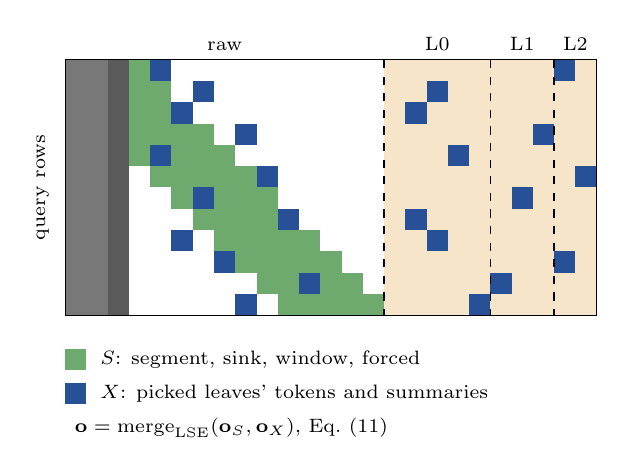
\begin{tikzpicture}[x=0.27cm,y=0.27cm,font=\scriptsize]
  % key axis: raw (0..14) | L0 (15..19) | L1 (20..22) | L2 (23..24); query rows 0..11 (top to bottom)
  \def\R{12}
  % causal raw band: full blocks for pinned (0..1), sink (2), window band
  \fill[cpin] (0,0) rectangle (2,-\R);
  \fill[csink] (2,0) rectangle (3,-\R);
  \foreach \r in {0,...,11} {
    \pgfmathsetmacro\a{max(3,\r+3-4)}
    \pgfmathsetmacro\b{\r+3+1}
    \fill[cwin] (\a,-\r) rectangle (\b,-\r-1);
  }
  % summary regions: structured runs of forced summaries are light
  \fill[csum!40] (15,0) rectangle (20,-\R);
  \fill[csum!40] (20,0) rectangle (23,-\R);
  \fill[csum!40] (23,0) rectangle (25,-\R);
  % X: scattered selected keys
  \foreach \r/\c in {0/4,1/6,2/5,2/16,3/8,4/4,4/18,5/9,6/6,6/21,7/10,8/5,8/17,9/7,9/23,10/11,11/8,11/19,3/22,5/24,7/16,10/20,1/17,0/23}
     \fill[csel] (\c,-\r) rectangle ++(1,-1);
  \draw[line width=0.3pt] (0,0) rectangle (25,-\R);
  \foreach \x in {15,20,23} \draw[line width=0.5pt,dashed] (\x,0) -- (\x,-\R);
  \node[above] at (7.5,0) {raw};
  \node[above] at (17.5,0) {L0};
  \node[above] at (21.5,0) {L1};
  \node[above] at (24,0) {L2};
  \node[rotate=90,anchor=south] at (-0.3,-6) {query rows};
  % legend
  \fill[cwin] (0,-13.6) rectangle ++(1,-1); \node[anchor=west] at (1.2,-14.1) {$S$: segment, sink, window, forced};
  \fill[csel] (0,-15.2) rectangle ++(1,-1); \node[anchor=west] at (1.2,-15.7) {$X$: picked leaves' tokens and summaries};
  \node[anchor=west] at (0,-17.3) {$\mathbf{o}=\mathrm{merge}_{\mathrm{LSE}}(\mathbf{o}_S,\mathbf{o}_X)$, Eq.~(11)};
\end{tikzpicture}
\caption{The split of a query's visible keys for training with selection at every position.
Keys are ordered $[\text{raw}\mid\text{L0}\mid\text{L1}\mid\cdots]$. The structured part $S$
(gray, green, light orange) is what a row sees whatever is selected: the protected segment,
the sink, the raw window and previous chunk, and the forced summaries; it forms runs, so
FlexAttention computes it on full blocks. The selected part $X$ (dark) is a few hundred keys
per row and KV group scattered over the compressed history; as a block mask nearly every
block would be partial, so a gather kernel reads each row's own key list instead. The two
outputs are merged by their log-sum-exp (Eq.~\eqref{eq:lse}).}
\label{fig:sx}
\end{figure}

\subsection{Training with Selection at Every Position}
\label{sec:sx}

\para{A dense selection mask does not scale.}
The first implementation selected for every row and wrote the result into a dense $[T,T]$
visibility matrix per KV group before converting it to a FlexAttention block mask. At 32K this
took 198\,s and 124\,GB per step, 54\,s of it in mask construction, and it failed at 64K, where
$T^2$ exceeds int32 indexing. Shrinking the matrix would not help: a query block's 128 rows
select different leaves, whose union touches almost every key block of the compressed region,
so the block mask approaches dense attention with an element-wise mask.

\para{We split each row's keys into a structured part and a selected part.}
For a raw row $p$, the visible set of Eq.~\eqref{eq:visible} is the disjoint union of $S(p)$,
the keys visible whatever is selected (protected segment, sink, the raw tokens of forced
leaves, and, without coarse terms, the forced summaries), and $X(p)$, the keys the picks add
(the raw tokens of picked leaves and the picked or unpicked summaries). In the level-grouped
key order $S(p)$ consists of runs, which FlexAttention computes on full blocks; $X(p)$ is a few
hundred keys per row and KV group (Figure~\ref{fig:sx}). The two partial attentions are merged
exactly:
\begin{equation}
  \mathbf{o}_p = \frac{e^{\mathrm{lse}_S(p)}\,\mathbf{o}_S(p) + e^{\mathrm{lse}_X(p)}\,\mathbf{o}_X(p)}
                      {e^{\mathrm{lse}_S(p)} + e^{\mathrm{lse}_X(p)}},
  \label{eq:lse}
\end{equation}
where $\mathrm{lse}$ is the log-sum-exp of the logits of each part; FlexAttention returns it
with gradient.

\para{The selected part needs one batched selection kernel and one gather kernel.}
The selection kernel processes all rows and KV groups in one launch. Its free candidates at
level $\ell$ are the children of the picks one level up plus one contiguous id range below the
forced nodes, at most $4kG+3$ per row whatever the context length, already in ascending id
order, so no sort is needed. The gather kernel streams each row's key list with an online
softmax for all heads of the group; its backward recomputes the probabilities, accumulates
$\mathrm{d}\mathbf{q}$ per row and scatters $\mathrm{d}\mathbf{k}$, $\mathrm{d}\mathbf{v}$ and
$\mathrm{d}\beta$ with atomic adds. Gradients flow through both the output and the log-sum-exp.
The structured part's block mask is built once per forward and shared by all layers and by
gradient-checkpoint recomputation; its inlined \texttt{mask\_mod} requires $64\times64$ tiles,
because the default tiles need 415\,KB of shared memory against 227\,KB per SM on an H200.

\subsection{Replay in Stage 2}
\label{sec:replay}

\para{Response rows get their own attention call.}
The replay first built an $[H,T,T]$ block mask per layer for all rows. Prompt rows, however,
attend under the gist mask that is shared by all layers and heads, and only the response rows
attend to recorded keys. We therefore compute prompt rows with the model's shared gist block
mask and response rows in a second FlexAttention call with an $[H_{kv},R,T]$ mask, which made a
128K step about three times faster (Table~\ref{tab:opsd}). Response rows are padded to at least
256 masked rows, because in our PyTorch version the compiled FlexAttention backward is wrong
for queries of at most 128 rows once another shape has been compiled.

\para{Two memory fixes were needed at 128K.}
Building routing labels with a one-hot unit matrix is $O(T^2)$, 17\,GB per level at 128K; a
scatter-add over units removes it. Gradient-checkpoint recomputation appended each layer's
auxiliary loss a second time and kept its graph alive until the next step; keeping only the
first copy cut the backward peak at 78K from 47\,GB to 17\,GB in stage 2, and the stage-1 peak
at 32K from 73\,GB to 11.2\,GB.

% ======================================================================================
\section{Evaluation}
\label{sec:eval}

\subsection{Experimental Setup}

\para{Model and hardware.}
All measurements use Qwen2.5-0.5B-Instruct \citep{qwen2025qwen25} (24 layers, 14 query heads,
2 KV heads, head dimension 64) in bf16 on one H200 with batch size 1, $L=J=4$, $D=4$, sink
$s=3$, previous chunks $P=1$, and the raw window of 2 turns and at most 8K tokens. Decoding
uses $k=256$ with union merging and no coarse terms; stage 1 uses $k=16$
(Section~\ref{sec:stage1}). The main target
model, Qwen2.5-7B-Instruct-1M \citep{yang2025qwen1m}, is being brought up; its results will be
added.
% TODO(authors): 7B-1M numbers from #22 (stage 1 at 32K, 256K append + decode, OPSD at 128K).

\para{Data.}
Training uses nebius/SWE-rebench-openhands-trajectories \citep{badertdinov2025swerebench,
wang2025openhands}, 67K OpenHands trajectories in OpenAI-style tool-call format, rendered with
the Qwen2.5 chat template together with the segment labels. In a subsample of 200
trajectories the median length is 50.6K tokens and 97\% exceed 32K; OpenHands truncates 2.3\% of tool results
at 30,047 characters, which we keep. The converted set contains 1,187 trajectories of at
least 100K tokens, which supply the 128K training runs; a stage-2 prompt is the trajectory cut
at the start of an assistant turn, with the cut between 100K and 131K raw tokens. We hold out
6\% of issues by hash. Lengths beyond 128K
are evaluation-only: 20 held-out sequences of 164K--260K tokens and 20 of 960K--1,038K, each
concatenating one attempt per issue from several issues.

\subsection{Exactness Checks}
\label{sec:exact}

\para{Full expansion reproduces the base model.}
With untrained summaries inserted and every node unfolded, the mean reverse KL to the base
model on raw text is $5\times10^{-9}$ at 512 tokens and $3\times10^{-10}$ at 8K, with a maximum of
$6.4\times10^{-7}$ over all tokens. Making the untrained summaries visible as well (SG+SR) gives
3.2--5.0 nats, which shows why a summary must be trained before it is shown.

\para{Fast paths match their references.}
Kernels A and B select exactly the same node ids as the PyTorch reference at every layer, KV
group and level, for both merges, with and without coarse terms, and their attention output is
allclose for head dimensions 64 and 128; the CUDA-graph decode path is bit-identical to
\texttt{model.forward} over 30 teacher-forced steps at 158K. The hybrid stage-1 attention
matches the dense-mask reference to a relative difference of at most $5\times10^{-6}$ in the
loss and every parameter gradient (fp32), and on the real model at 8K the step-1 losses of the
two agree within 0.1\% in bf16.

\begin{table}[t]
\caption{Decode time per raw token (including the 0.33 summary tokens fed after each raw token
on average), with and without CUDA graphs for the dense parts, on Qwen2.5-0.5B, one H200, $k=256$, union, raw window 8K. Prompts are a held-out
256K trajectory cut to the given raw length.}
\label{tab:decode}
\centering\small
\begin{tabular}{lcccc}
\toprule
Raw & Gisted & Keys/layer & Graphs & No graphs \\
\midrule
128K & 172,704 & 12K--27K & \textbf{29.9}\,ms & 43.3\,ms \\
256K & 304,847 & 12K--27K & \textbf{30.8}\,ms & 43.6\,ms \\
\bottomrule
\end{tabular}
\end{table}

\begin{table}[t]
\caption{Decode step time on a 158K-token prompt (Qwen2.5-0.5B, H200, $k=256$) after each
optimization, applied in order. ``Exact'' means logits and recorded keys are bit-identical to
the previous row.}
\label{tab:decode_steps}
\centering\small
\begin{tabular}{p{4.7cm}cc}
\toprule
Change & Step (ms) & Exact \\
\midrule
Starting point & 141 & -- \\
Kernel B splits scale with the key list & 120 & --$^{a}$ \\
Raw rows skip summary LoRA and $\beta$ & 109 & yes \\
Layer 0 and summary rows on kernel B & 81 & no$^{b}$ \\
Next-level candidates in one kernel & 57 & yes \\
Pick: one program per head$^{c}$ & 57 & yes \\
Skip per-step $O(T)$ mask construction & 55 & yes \\
Key list in one kernel; top level once per step & 46 & yes \\
Dense parts as CUDA graphs & 33 & yes \\
\bottomrule
\end{tabular}

\vspace{2pt}
\raggedright\footnotesize
$^{a}$Run-to-run deterministic. $^{b}$Same argmax at every step; mean log-probability
difference 0.043 (bf16 level); identical layer-0 key sets. $^{c}$GPU time 41$\to$22\,ms; the
step became launch-bound.
\end{table}

\subsection{Inference Efficiency}

\para{Decode latency is nearly flat from 128K to 256K.}
Doubling the raw context from 128K to 256K raises the per-token time from 29.9\,ms to 30.8\,ms
with CUDA graphs and from 43.3\,ms to 43.6\,ms without (Table~\ref{tab:decode}), because each
layer reads only the 12K--27K selected keys. We estimate the read volume at about 180\,MB per
token at 128K, against about 2.1\,GB for dense attention; at H200 bandwidth this is tens of
microseconds, so the step is bound by kernel launches and host work rather than memory traffic.
% TODO(authors): measured read volume, and a dense FlashAttention/FlashDecoding baseline at
% the same lengths for the same model.

\para{Appending a long tool result is no longer the bottleneck of a turn.}
Grouping summary keys by level cuts a 158K append from 57.1\,s to 11.1\,s after warm-up, and
the first append of a process, which includes compilation, from 86\,s to 40\,s
(Table~\ref{tab:prefill}). The remaining partial blocks come from summary rows interleaved
with raw rows in the query order; reordering queries the same way is estimated to give a
further $1.5\times$ at most.

\begin{table}[t]
\caption{Appending a 158K-token agent prompt in one piece (Qwen2.5-0.5B, H200). Block counts
are over the causal grid of 128-token blocks.}
\label{tab:prefill}
\centering\small
\begin{tabular}{lcc}
\toprule
& Sequence order & Grouped by level \\
\midrule
Partial blocks & 209,930 (27.6\%) & 39,596 (5.2\%) \\
Full blocks & 53,262 & 54,257 \\
Append, warm & 57.1\,s & \textbf{11.1}\,s \\
Append, first call & 86\,s & 40\,s \\
\bottomrule
\end{tabular}
\end{table}

\subsection{Training Efficiency}

\para{Stage 1 with selection at every position trains at 128K.}
With the structured/selected split, a step takes 35\,s and 11.2\,GB at 32K, 74.5\,s and 20\,GB at
64K, and 174\,s and 37.8\,GB at 128K, close to linear in both (Table~\ref{tab:stage1}). The dense
selection mask took 198\,s and 124\,GB at 32K and failed at 64K. The first step additionally
pays 214--493\,s of compilation.

\begin{table}[t]
\caption{Stage-1 step time and peak memory with selection at every position (Qwen2.5-0.5B,
H200, batch 1, agent trajectories, $k=16$, $D=4$, raw window 8K; steady state). Dense: the
selection written to a $[T,T]$ mask; split: FlexAttention over $S$ plus gather over $X$.}
\label{tab:stage1}
\centering\small
\begin{tabular}{lcccc}
\toprule
& \multicolumn{2}{c}{Dense mask} & \multicolumn{2}{c}{Split $S$/$X$} \\
\cmidrule(lr){2-3}\cmidrule(lr){4-5}
Length & Step & Memory & Step & Memory \\
\midrule
16K  & 49\,s$^{a}$ & 47\,GB & -- & -- \\
32K  & 198\,s & 124\,GB & \textbf{35}\,s & \textbf{11.2}\,GB \\
64K  & fails$^{b}$ & -- & 74.5\,s & 20\,GB \\
128K & -- & -- & 174\,s & 37.8\,GB \\
\bottomrule
\end{tabular}

\vspace{2pt}
\raggedright\footnotesize
$^{a}$Mean of 4 steps including the first, compiled step. $^{b}$Illegal memory access: $T^2$
exceeds int32 indexing at about 80K gisted tokens.
\end{table}

\para{Stage 2 at 128K takes under a minute per step.}
Table~\ref{tab:opsd} follows one step of OPSD at 128K through the fixes of
Sections~\ref{sec:prefill} and~\ref{sec:replay}. Moving response rows to their own attention
call cut steps from 571--1,086\,s to 172--302\,s; the level-grouped key order then cut the
rollout's append, and a 133K-context step to 54.7\,s, of which the rollout is 22.6\,s. Memory
stays at 33--38\,GB. Interrupted runs resume from their checkpoints.

\begin{table}[t]
\caption{Stage-2 (OPSD) step time at 128K (Qwen2.5-0.5B, H200, batch 1, 128 generated tokens
per step, prompts of 100K--131K raw tokens, i.e. 133K--158K with summaries; same samples across
rows; peak memory 33--38\,GB).}
\label{tab:opsd}
\centering\small
\begin{tabular}{p{4.6cm}c}
\toprule
Implementation & Step \\
\midrule
Replay with an $[H,T,T]$ mask per layer & 571--1,086\,s \\
Response rows in their own call & 172--302\,s \\
\ \ + summary keys grouped by level (133K) & \textbf{54.7}\,s \\
\bottomrule
\end{tabular}
\end{table}

\subsection{Quality}
\label{sec:quality}

% Quality results do not exist yet in the agent setting. Every cell below is TBD.

\para{Suffix KL to the full-attention teacher.}
The development metric is the mean per-token KL, on held-out trajectories, between the student
and the base model reading the raw text, over each assistant turn (Table~\ref{tab:kl}).

\begin{table}[t]
\caption{Mean per-token KL (nats) to the full-attention base model on held-out agent
trajectories, by context length.}
\label{tab:kl}
\centering\small
% Will hold: suffix / per-turn KL vs the full-attention teacher for each checkpoint, at 32K, 128K, 256K
% (and 1M for the structure check), held-out split of experiments/agent_data.py and #23.
\begin{tabular}{lcccc}
\toprule
Checkpoint & 32K & 128K & 256K & 1M \\
\midrule
Stage 1 (no selection) & \tbd & \tbd & \tbd & \tbd \\
Stage 1 (selection) & \tbd & \tbd & \tbd & \tbd \\
+ Stage 2 (OPSD) & \tbd & \tbd & \tbd & \tbd \\
\bottomrule
\end{tabular}
\end{table}

\para{Training-time selection gate.}
Table~\ref{tab:gate} records the pre-registered comparison of stage 1 with and without
selection at every position, evaluated with unfolding at decode only or at every suffix
position.

\begin{table}[t]
\caption{Selection gate: stage 1 without (A) and with (B) selection at every position, same
data, steps and seed; KL on 8K (and 32K) held-out sequences, passkey accuracy by key position.}
\label{tab:gate}
\centering\small
% Will hold: the #28 gate at 8K and its #29 repeat at 32K on agent trajectories
% (suffix KL, passkey front / back half). Withheld until the 32K repeat's training issue is resolved.
\begin{tabular}{llccc}
\toprule
Train & Unfold at & Suffix KL & Front & Back \\
\midrule
A & decode & \tbd & \tbd & \tbd \\
A & every position & \tbd & \tbd & \tbd \\
B & decode & \tbd & \tbd & \tbd \\
B & every position & \tbd & \tbd & \tbd \\
\bottomrule
\end{tabular}
\end{table}

\para{Retrieval and agent tasks.}
Retrieval is measured by passkey and RULER-style \citep{hsieh2024ruler} tasks with the key at
controlled depths, and agent quality by task success on held-out issues at milestones
(Table~\ref{tab:tasks}).

\begin{table}[t]
\caption{Retrieval accuracy and agent task success.}
\label{tab:tasks}
\centering\small
% Will hold: passkey / RULER-style retrieval by depth and length (32K-256K), and agent task
% success on held-out issues, for base (full attention), stage 1, OPSD.
\begin{tabular}{lccc}
\toprule
Model & Passkey & RULER & Task success \\
\midrule
Base (full attention) & \tbd & \tbd & \tbd \\
Stage 1 & \tbd & \tbd & \tbd \\
+ OPSD & \tbd & \tbd & \tbd \\
\bottomrule
\end{tabular}
\end{table}

\para{Ablations.}
The selector's switches and the parameterization are ablated on the same model and data
(Table~\ref{tab:ablation}).

\begin{table}[t]
\caption{Ablations at a fixed budget.}
\label{tab:ablation}
\centering\small
% Will hold: KL and retrieval for union vs sumexp, coarse terms off/on, k per level, routing
% KL scope (level vs oracle children), fanout 4 vs 8/16, depth D, beta (none/level/content),
% LoRA on summary rows vs all rows, training k vs inference k, candidate-local positions above 256K (#27).
\begin{tabular}{lcc}
\toprule
Variant & KL & Retrieval \\
\midrule
Default (union, no coarse terms) & \tbd & \tbd \\
Sumexp merge & \tbd & \tbd \\
Coarse terms (exact partition) & \tbd & \tbd \\
Wider beam at upper levels & \tbd & \tbd \\
Routing KL over oracle children & \tbd & \tbd \\
Fanout 8 / 16 & \tbd & \tbd \\
No content term in $\beta$ & \tbd & \tbd \\
LoRA on all rows & \tbd & \tbd \\
Training $k$ = inference $k$ & \tbd & \tbd \\
\bottomrule
\end{tabular}
\end{table}

% ======================================================================================
\section{Limitations}

\para{Two limitations are inherent to the design.}
Appended tokens read old content only through summaries, so the keys and values of a long
tool result are computed from a compressed view of the history; any design that prefills
without unfolding pays this, and its cost will be measured with the quality results. Union
merging lets the budget grow with the number of heads per group, up to $Gk$ nodes per level;
sumexp bounds it at $k$ at the price of one shared ranking per group.

\para{The current implementation also has limits that are not inherent.}
Decoding is batch 1 and keeps all keys and values on the GPU; for 7B at 1M and batch 1 we
estimate 92\,GB on an H200 (15\,GB weights, 57\,GB raw KV, 20\,GB summary KV), and offloading raw
keys and values to host memory is deferred. Only the dense part of a decode step is captured in
CUDA graphs. The stage-2 replay mask is $[H_{kv},R,T]$ booleans per layer, about 350\,MB at 128K
with 1K generated rows, which would grow to about 4\,GB per layer for 7B at 1M. Response rows are
padded to 256 to avoid a FlexAttention backward bug. Kernel A writes scores to a scratch buffer
rather than keeping them on chip. The existing SSA decode path in bf16 is not run-to-run
deterministic on H200, which limits byte-level regression checks against it.

\section{Conclusion}

\ours stores a trajectory's history as a streaming 4-ary tree of learned summary tokens and
lets each query descend it with a fixed beam per level, so that the keys a decode step reads
stay nearly constant as the trajectory grows, while full expansion remains exactly the frozen
base model. Training distills each tree level into the one below and then distills on the
student's own rollouts; the kernels that make append, decode and training-time selection
practical bring a 128K decode step to 30\,ms and a 128K stage-1 step to 3 minutes on a 0.5B
model. Whether the summaries keep the base model's quality at 128K--256K is the open question
the next experiments answer.

\bibliographystyle{plainnat}
\bibliography{refs}

\end{document}
